%! Author = Antonio Lobo
%! Date = 30/10/2024

\subsection{Reduction Methods}
In this section, we briefly describe reduction techniques employed for instance-based learning. We use a simple 2D dataset for illustrative purposes.

\subsubsection{GCNN}

The Generalized Condensed Nearest Neighbor (GCNN) algorithm is an extension of the traditional Condensed Nearest Neighbor (CNN) method, which incorporates adaptive prototype learning approach. This is an \textbf{undersampling} technique which try to find a subset of prototypes $U \subseteq X$, where $X = \{(x_1,y_1), \ldots, (x_n,y_n)\}$ is our dataset, that correctly represents our data. This is specially beneficial for unbalanced datasets. The main idea behing CNN is to select prototypes that \textit{absorbe} points that can be represented using that protype. Let's break down the steps for this method:

\begin{enumerate}
	\item \textbf{Prototype selection:} In this step we need to select a prototype for each class. So for each class $c_j$, let $X_j= \{ (x,y) : y=c_j\}$ be all the elements of this class. We will select as a prototype $x_j^*$ that is the nearest neighbor of most points of its class, thus it will influence the most points in any KNN. i.e. : 
	$$
	x_j^* = \arg\max_{x \in X_j} \left( \sum_{x' \in X_j \setminus \{x\}}\left(x = \operatorname{NN}_{X_j \setminus \{x'\}}(x')\right) \right)
	$$
	So we will have $U = \{ x_j^* : j = 1,\ldots, m \}$ and we will denote as $U_j$ all the prototypes of class $c_j$.
	
	\item \textbf{Absorbtion:} This is one of the key differences with CNN, first let define $\delta_n = \min_{\{ (x_i,y_i), (x_j, y_j) \in X : y_i \neq y_j\}}\}\left( \|x_i - x_j\| \right)$ , for every point $x_i$ let $p = \arg\min_{x \in U_j}\left( ||x-x_i|| \right)$ and $q = \arg\min_{x \in \left( U \setminus U_j \right)}\left( ||x-x_i|| \right)$ be the nearest protoypes of the same class and other class respectively. We will absorb $x_i$ if it satisfy the following condition:
	$$
	\| \mathbf{x} - \mathbf{q} \| - \| \mathbf{x} - \mathbf{p} \| > \rho \delta_n, \quad \rho \in [0, 1).
	$$
	With CNN being $\rho=0$, this means that if the $x_i$'s closest prototype is of its class, it will be absorbed. $\rho$ variables just introduces a slack for this decission illustrated in \textbf{Figure} \ref{fig:gcnnRhoIllustration}
	
	\begin{figure}[ht]
		\centering
		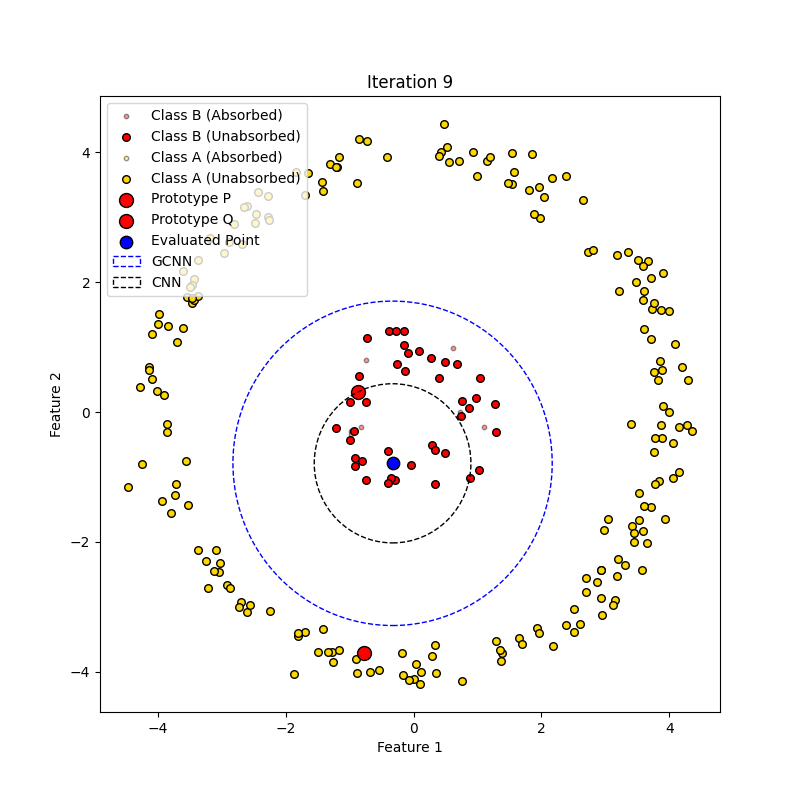
\includegraphics[width=0.5\textwidth]{figures/gcnn/gcnnRhoIllustration}
		\caption{Effect of Rho in GCNN Illustrated}
		\label{fig:gcnnRhoIllustration}
	\end{figure}
	
	\item \textbf{Prototype Augmentation:} If there are still points that haven't been absorbed for class $c_j$, we will repeat the prototype selection but only taking into account unabsorbed points and then go to step 2 again. If all points have been absorved we finish the process.
\end{enumerate}

In \textbf{Figures} \ref{fig:rho_variation_1} and \ref{fig:rho_variation_2} we illustrate the effect of this method in a specially constructed dataset where we can clearly see it with $\rho$ varying froom 0 to 1.

\begin{figure}[htbp]
	\centering
	\begin{subfigure}[b]{0.3\textwidth}
		\centering
		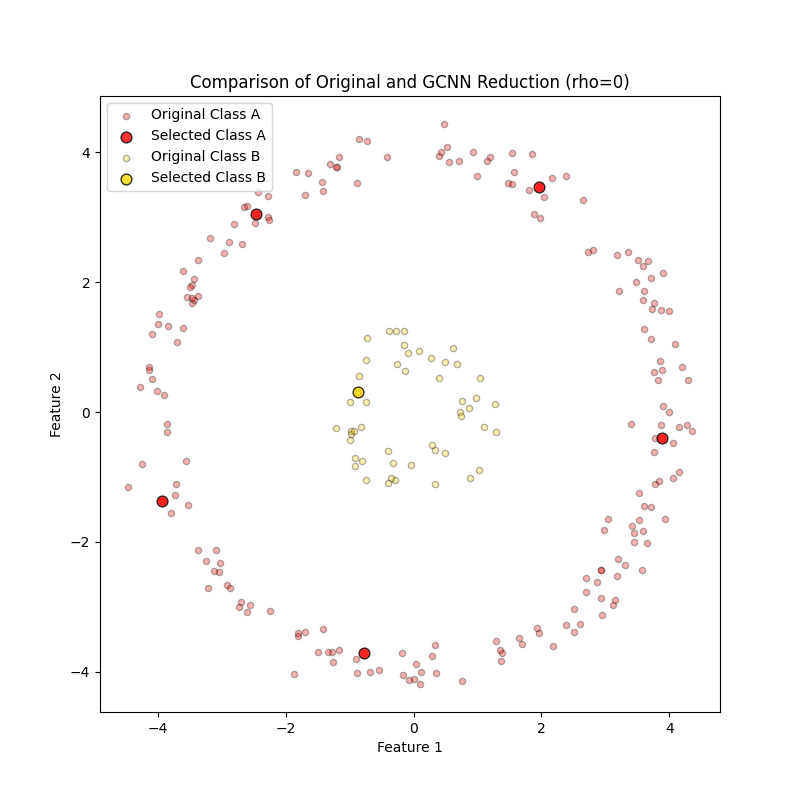
\includegraphics[width=\textwidth]{figures/gcnn/comparison_plot_rho_0.png}
		\caption{$\rho = 0$}
		\label{fig:rho0}
	\end{subfigure}
	\hfill
	\begin{subfigure}[b]{0.3\textwidth}
		\centering
		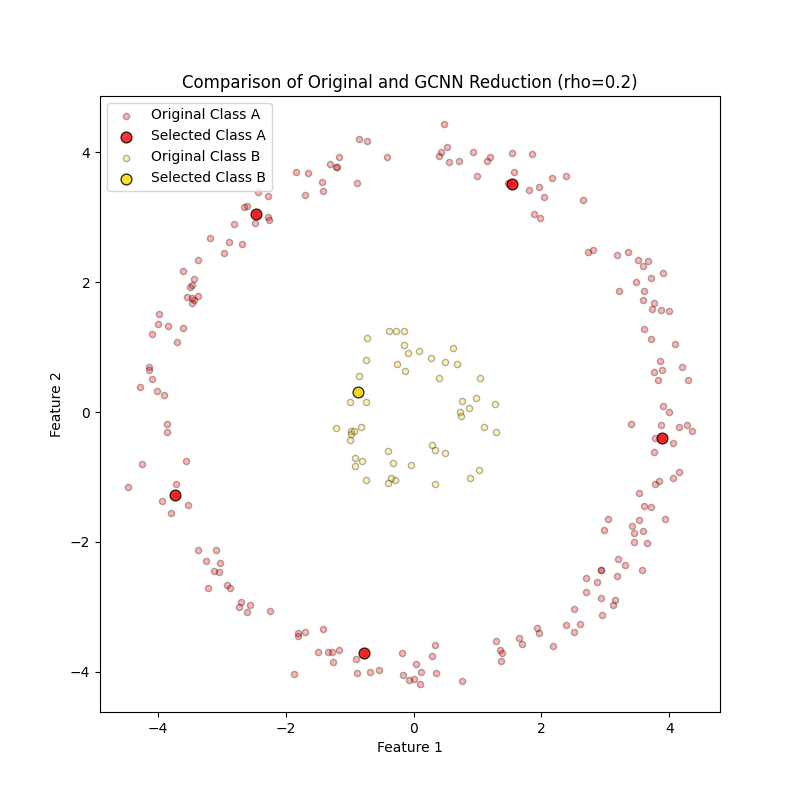
\includegraphics[width=\textwidth]{figures/gcnn/comparison_plot_rho_0.2.png}
		\caption{$\rho = 0.2$}
		\label{fig:rho0.2}
	\end{subfigure}
	\hfill
	\begin{subfigure}[b]{0.3\textwidth}
		\centering		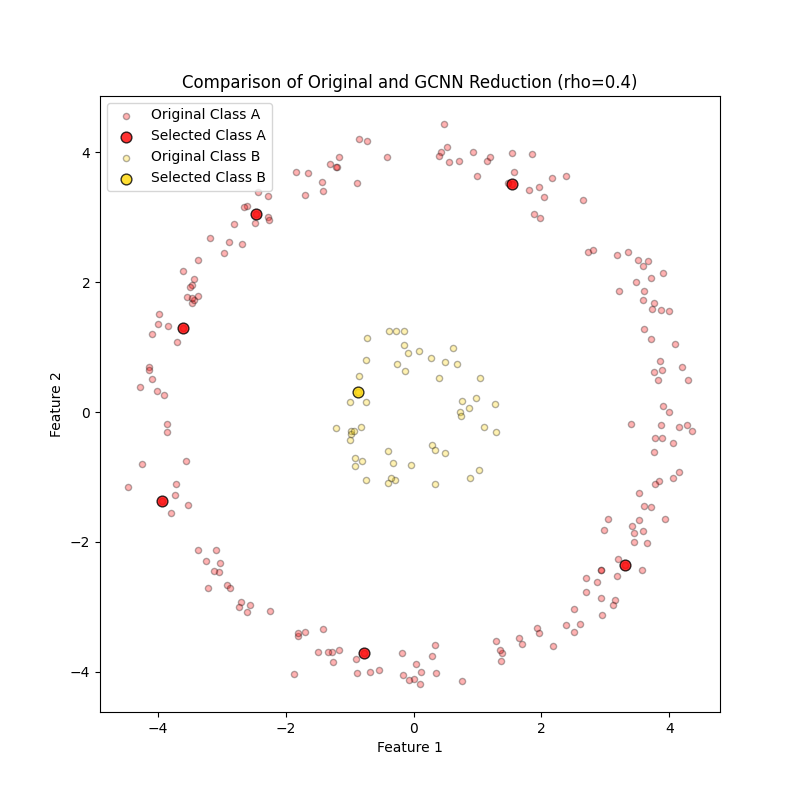
\includegraphics[width=\textwidth]{figures/gcnn/comparison_plot_rho_0.4.png}
		\caption{$\rho = 0.4$}
		\label{fig:rho0.4}
	\end{subfigure}
	\caption{GCNN illustration $\rho=0.6,0.8,1$}
	\label{fig:rho_variation_1}
\end{figure}

% Second Figure with the remaining 3 subfigures
\begin{figure}[htbp]
	\centering
	\begin{subfigure}[b]{0.3\textwidth}
		\centering
		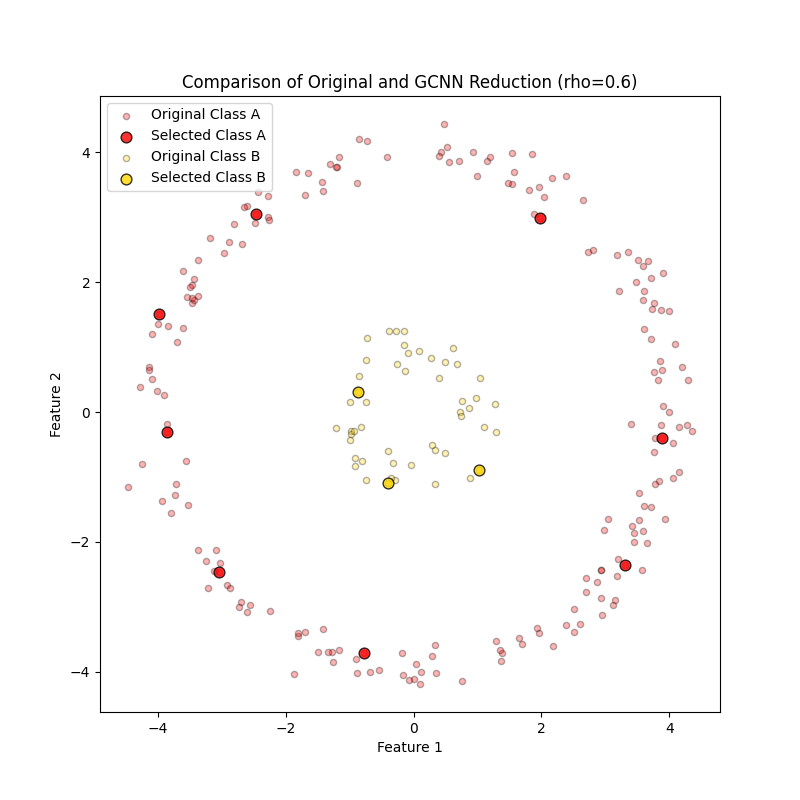
\includegraphics[width=\textwidth]{figures/gcnn/comparison_plot_rho_0.6.png}
		\caption{$\rho = 0.6$}
		\label{fig:rho0.6}
	\end{subfigure}
	\hfill
	\begin{subfigure}[b]{0.3\textwidth}
		\centering
		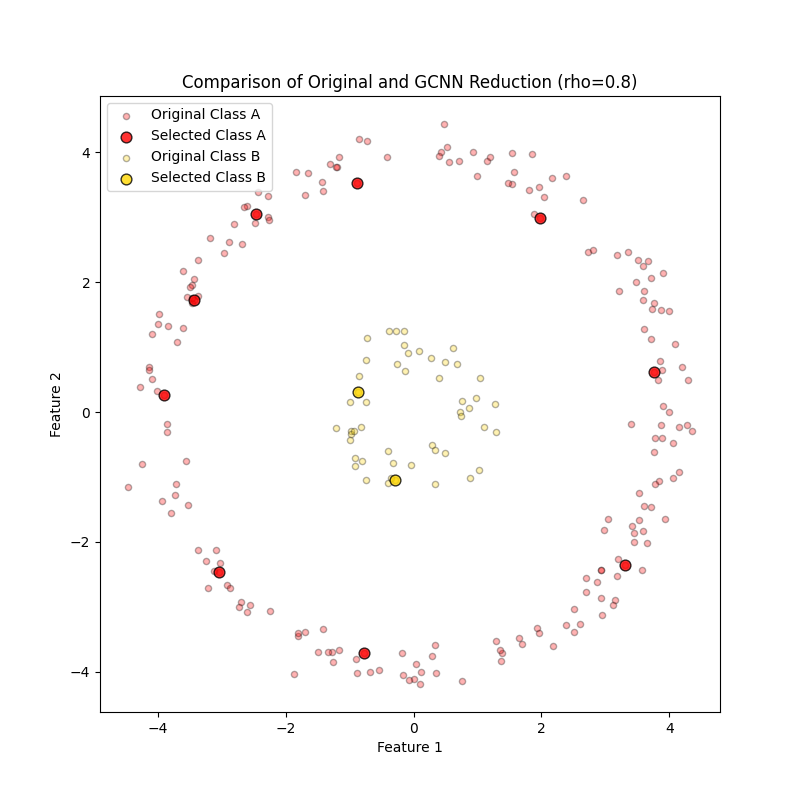
\includegraphics[width=\textwidth]{figures/gcnn/comparison_plot_rho_0.8.png}
		\caption{$\rho = 0.8$}
		\label{fig:rho0.8}
	\end{subfigure}
	\hfill
	\begin{subfigure}[b]{0.3\textwidth}
		\centering
		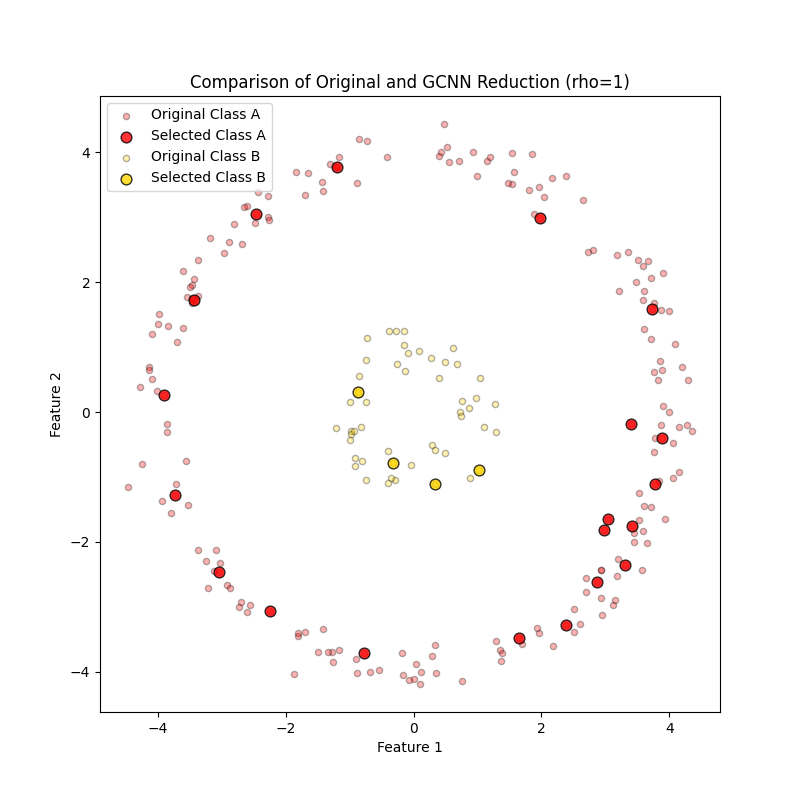
\includegraphics[width=\textwidth]{figures/gcnn/comparison_plot_rho_1.png} % Add the new plot here
		\caption{$\rho = 1$}
		\label{fig:rho1}
	\end{subfigure}
	\caption{GCNN illustration $\rho=0.6,0.8,1$}
	\label{fig:rho_variation_2}
\end{figure}


\subsubsection{EENTH}
This subsection outlines the Elimination Editing with Nearest-neighbor Threshold (EENTH) method \cite{vazquez2005}. This approach uses a modified $k$-NN rule, integrating probability-based decisions for instance elimination. The main steps are outlined below.

\begin{enumerate}
	\item \textbf{Probability-based Classification}: For each instance $ x $, calculate the probability $ p_i(x) $ of $ x $ belonging to each class $ i $ based on its $k$-nearest neighbors. Probabilities are weighted inversely by the distance to each neighbor and normalized:
	
	
	\begin{center}
		\begin{align}
			p_i^j &= \frac{|\{x_k \in NN_k(x) : y_k=j \}|}{k} \\
			P_i(x) &= \sum_{j=1}^{k} p_i^j \frac{1}{1 + d(x, x^j)} \\
			p_i(x) &= \frac{P_i(x)}{\sum_{j=1}^{M} P_j(x)}
		\end{align}
	\end{center}
	
	
	\item \textbf{Thresholding}: Define a threshold $ \mu $ to refine classification, we will denote as $p(x)$ the highest probability. Instances near decision boundaries, where $ p(x) < \mu $, are identified as candidates for removal.
	
	\item \textbf{Elimination}: If an instance $ x $ does not match the class with the highest probability, or if its highest class probability falls below $ \mu $, it is removed from the dataset, resulting in an edited set $ S \subseteq X $.
\end{enumerate}

The EENTH method thus provides a balance between retaining instances with high classification confidence and discarding uncertain instances near decision boundaries. Best values for $\mu$ are dependent on the dataset, In \textbf{Figures} \ref{fig:mu_variation_1, fig:mu_variation_2} we illustrate the results for $\mu$ varying from 0.15 to 0.85 taking 5 neighbors into account.

\begin{figure}[htbp]
	\centering
	\begin{subfigure}[b]{0.3\textwidth}
		\centering
		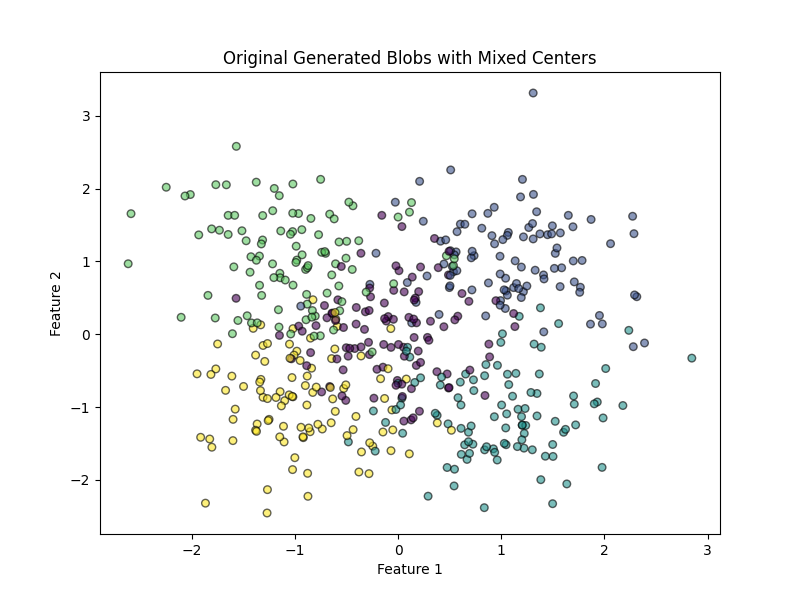
\includegraphics[width=\textwidth]{figures/eenth/original_blobs}
		\caption{Original}
		\label{fig:original}
	\end{subfigure}
	\hfill
	\begin{subfigure}[b]{0.3\textwidth}
		\centering
		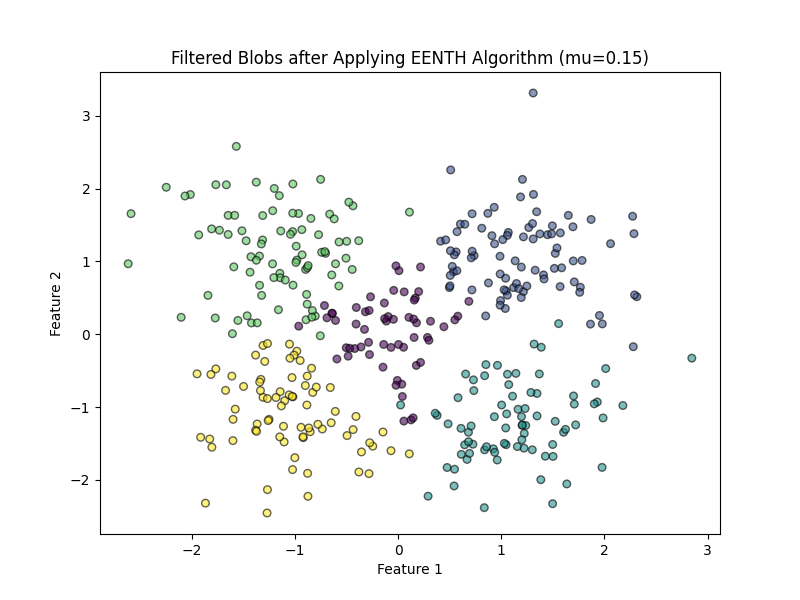
\includegraphics[width=\textwidth]{figures/eenth/filtered_blobs_mu_0.15}
		\caption{$\mu = 0.2$}
		\label{fig:mu0.2}
	\end{subfigure}
	\hfill
	\begin{subfigure}[b]{0.3\textwidth}
		\centering
		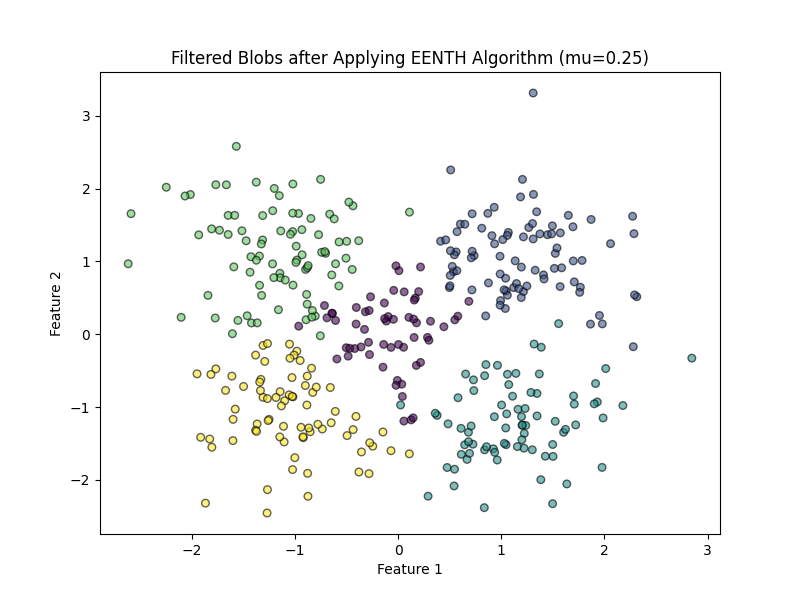
\includegraphics[width=\textwidth]{figures/eenth/filtered_blobs_mu_0.25}
		\caption{$\mu = 0.4$}
		\label{fig:mu0.4}
	\end{subfigure}
	\caption{Illustration of dataset after applying EENTH method with $\mu$ values 0.15 and 0.25.}
	\label{fig:mu_variation_1}
\end{figure}

% Second Figure with the remaining 3 subfigures
\begin{figure}[htbp]
	\centering
	\begin{subfigure}[b]{0.3\textwidth}
		\centering
		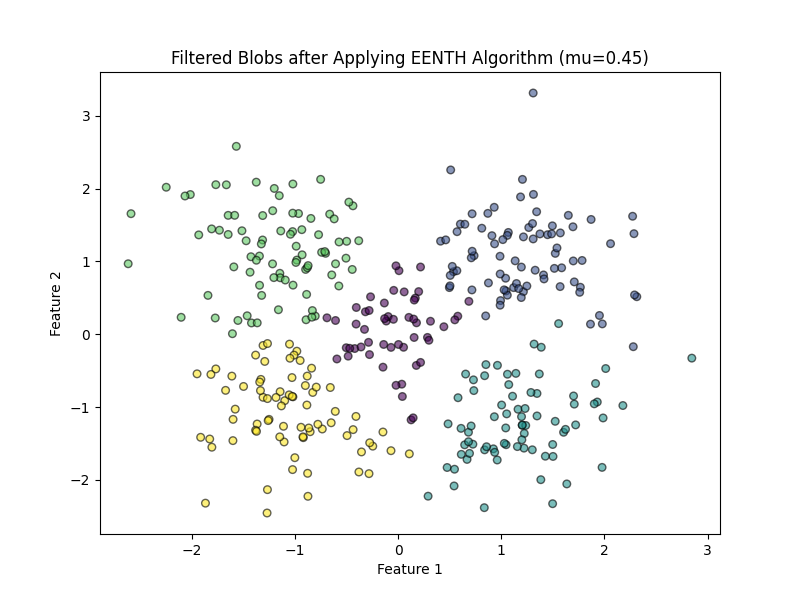
\includegraphics[width=\textwidth]{figures/eenth/filtered_blobs_mu_0.45}
		\caption{$\mu = 0.45$}
		\label{fig:mu0.45}
	\end{subfigure}
	\hfill
	\begin{subfigure}[b]{0.3\textwidth}
		\centering
		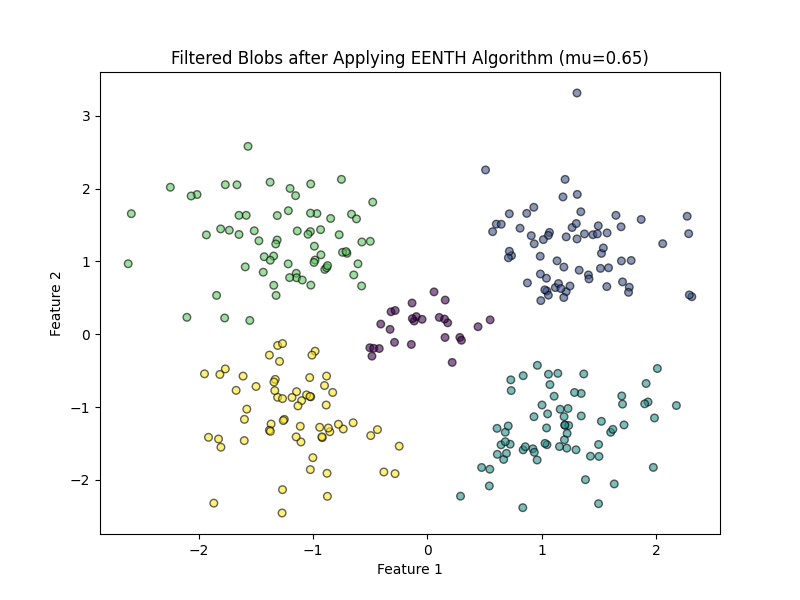
\includegraphics[width=\textwidth]{figures/eenth/filtered_blobs_mu_0.65}
		\caption{$\mu = 0.65$}
		\label{fig:mu0.65}
	\end{subfigure}
	\hfill
	\begin{subfigure}[b]{0.3\textwidth}
		\centering
		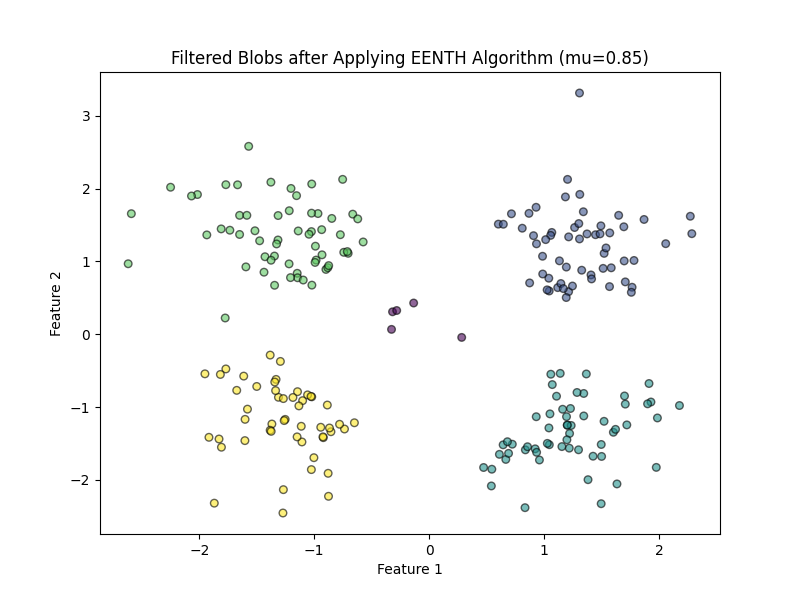
\includegraphics[width=\textwidth]{figures/eenth/filtered_blobs_mu_0.85} % Add the new plot here
		\caption{$\mu = 0.85$}
		\label{fig:85}
	\end{subfigure}
	\caption{EENTH illustration $\mu=0.45,0.65,0.85$}
	\label{fig:mu_variation_2}
\end{figure}




\subsubsection{DROP3}
In this subsection, we describe the basic concepts of the third method in the Decremental Reduction Optimization Procedure (DROP) family, as presented in Section 3 of Wilson et al. \cite{wilson2000reduction}. Although we will not delve into every detail, we describe the main ideas of the algorithm and illustrate them on $D_1$. See \textbf{Figure} \ref{fig:2dDataset}.

\begin{enumerate}
	\item \textbf{Remove noise}: The first step is to remove noisy instances using Edited Nearest Neighbor (EEN) \cite{wilson1972asymptotic}, where any instance misclassified by its $ k $-nearest neighbors is removed. The outcome of applying this technique is shown in \textbf{Figure} \ref{fig:2dEEN}, where noise has been removed. We denote the reduced dataset as $ T \subseteq D_1 $.
	\begin{figure}[ht]
		\centering
		\begin{minipage}{0.45\textwidth}
			\centering
			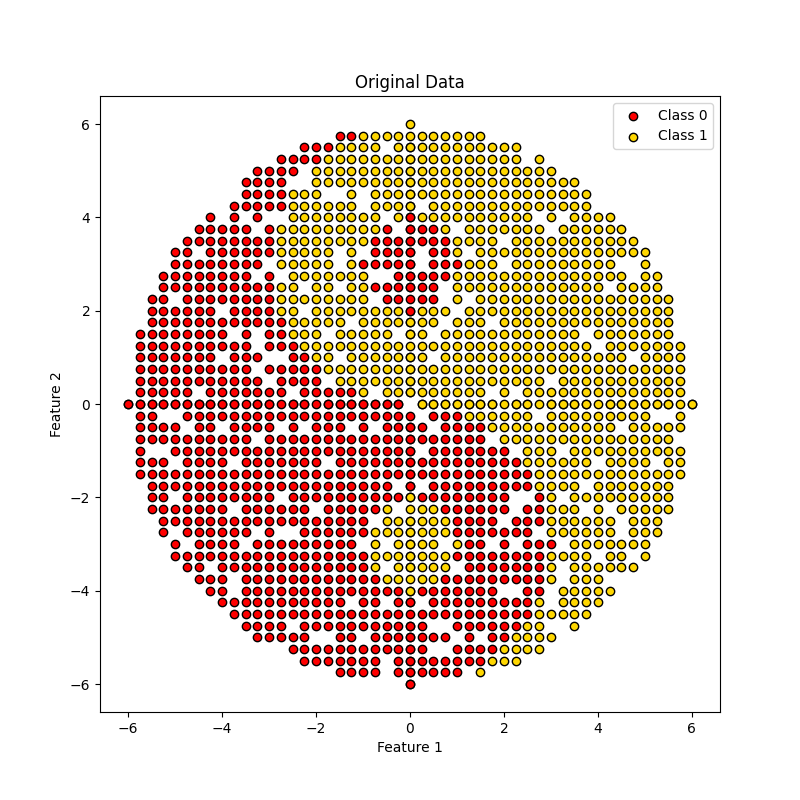
\includegraphics[width=\textwidth]{figures/DROP3/2dDataset} % Adjust path and file name
			\caption{Original Dataset}
			\label{fig:2dDataset}
		\end{minipage}\hfill
		\begin{minipage}{0.45\textwidth}
			\centering
			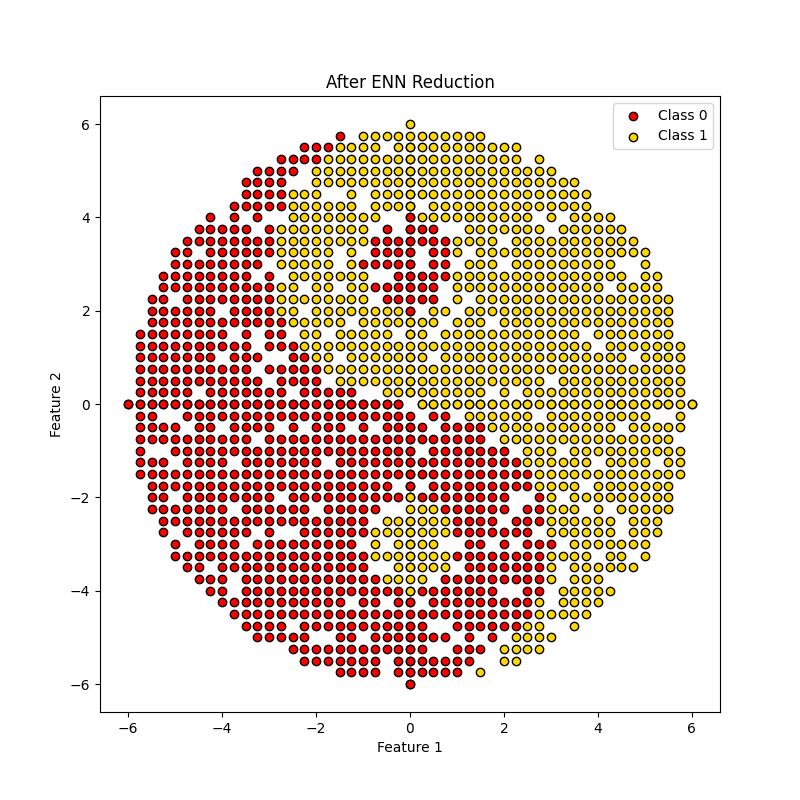
\includegraphics[width=\textwidth]{figures/DROP3/2dEEN} % Adjust path and file name
			\caption{Effect of EEN}
			\label{fig:2dEEN}
		\end{minipage}
	\end{figure}
	
	\item \textbf{Sort points}: The next step is to prioritize removing points that are farthest from the decision boundary. For each point $ x_i \in S $ with class $ y_i $, we compute the distance to the nearest point with a different class, denoted as $ x_j \in D $ such that $ y_j \neq y_i $ and $ \nexists x_k : |x_k - x_i| < |x_j - x_i| \land y_i \neq y_k $.
	
	\item \textbf{Delete points}: Let $ S = T $. Starting with the points farthest from the boundary, we check if any associated points (points that have $ x_i $ as a neighbor) $ a_j $ receive more votes for their correct class with $ x_i $ as a neighbor (denoted as $ \text{with} $) or if they would be classified correctly if $ x_i $ were removed (denoted as $ \text{without} $). If $ \text{without} > \text{with} $, we remove $ x_j $ from $ S $, resulting in $ S' = S \setminus \{x_j\} $.
	
	\item \textbf{Selecting neighbors}: A key distinction between DROP1 and DROP2 is that DROP1 removes points that are removed from the dataset from the list of associates while DROP2 doesn't.
	
	\begin{figure}[ht]
		\centering
		\begin{minipage}{0.45\textwidth}
			\centering
			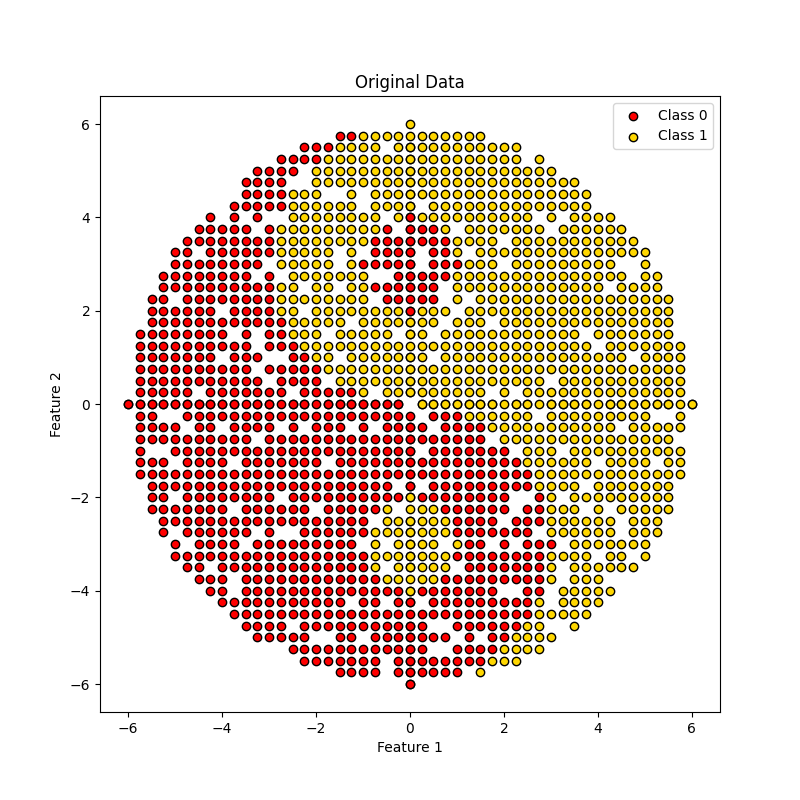
\includegraphics[width=\textwidth]{figures/DROP3/2dDataset} % Adjust path and file name
			\caption{Original Dataset}
			\label{fig:2dDataset2}
		\end{minipage}\hfill
		\begin{minipage}{0.45\textwidth}
			\centering
			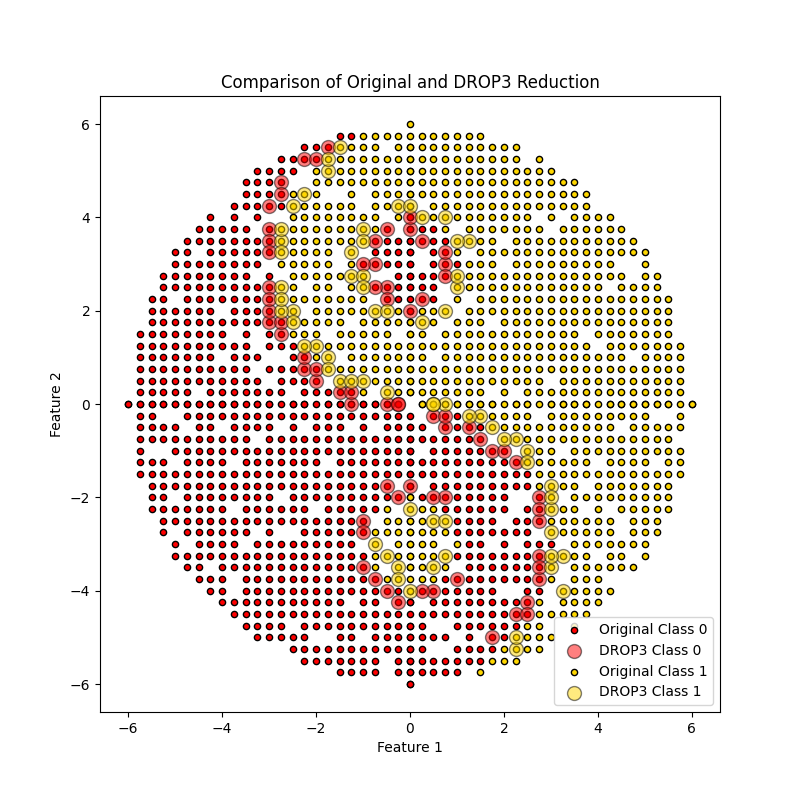
\includegraphics[width=\textwidth]{figures/DROP3/DROP3} % Adjust path and file name
			\caption{Effect of DROP3}
			\label{fig:DROp3Total}
		\end{minipage}
	\end{figure}
	
\end{enumerate}
